
\normalsize\chapter{METHODOLOGY}

\section{Introduction}
\par This chapter discusses the methodology that was used in gathering the data and
implementing a RFID Based Surveillance System. Here the researcher aimed at identi
fying the objectives to be carried out and the methods and tools to be used to
present and analyze data to develop the RFID Based Surveillance System.\\
\section{Data Collection Techniques}

%\begin{figure}
%    \centering
%    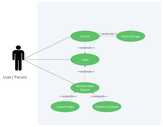
\includegraphics{b1.jpg}
%    \caption{Block diagram of waste classification}
%    \label{Block diagram of waste classification}
%\end{figure}
\subsection{Interviews}
An interview is a process of conducting intensive individual interviews with a small
number of respondents to explore their perspectives on a particular idea, program
or situation. Face to face method of discussion was used to gather information
from people who work in the company / organization and get the knowledge to
design a responsive system.
\subsection{Observation}
This technique was used to gather accurate information about how the system
actually operates, particularly about processes. This involves the researcher to
systematically watch and record the behaviors and characteristics of operations
and processes in the company. Although the method is time consuming, it has a
number of advantages, which include: It gives more detailed and context related
information, It permits the collection of information on facts not mentioned in the
interview, It permits tests of the reliability of the responses to the questionnaires,
observe operations of a program as they are actually occurring and can adapt to
events as they occur.
\subsection{Design}
In systems design the design functions and operations are described in detail, in-
cluding business rules, process diagrams and other documentation. The output of
this stage was describe the new system as a collection of modules or subsystems.
The design stage takes as its initial input the requirements identified in the ap-
proved requirements document. For each requirement, a set of one or more design
elements will be produced as a result of interviews, workshops, and/or prototype
efforts.

%\begin{figure}
%    \centering
%    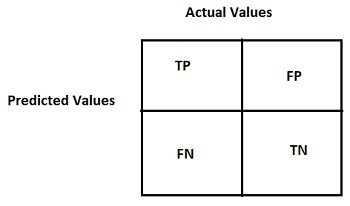
\includegraphics{v7.jpg}
%    \caption{Confusion Matrix}
%    \label{Confusion Matrix}
%\end{figure}
\section{Study Findings}
\par According to the data collection methods the following was thought to be done to
improve on the gaps found in the current system.
\subsection{Weakness of the Current System}
It was through the information got about the current system that the researcher
was able to identify its weaknesses. This helped in understanding what was to be
done in order to develop a new system.\\
The following weaknesses were found in the current system:
\begin{itemize}
    \item In the current system parents don't have access to view the footage of the bus.
\item There is no system for identifying students. So, Outsiders can also be travel through the bus without any problem.
\item The current system is very costly and not efficient.
\item Parents don't have the permission to download the bus footages.
\end{itemize}
\subsection{Presentation and Analysis of the findings}
\par From the analysis made, there is need for an online RFID Based Surveillance System to enusure safety to students with more features and functionalities. The current system is unreliable, inefficient and costly. Three
categories of stakeholders were interviewed and these included;
\section{Designing or modeling the system}
System design tools to create systems that meet the needs of parants.The
tools are used in system designing and modeling are flow charts, use case diagrams. A system flow chart is a way
of displaying how data flows in a system and how decisions are made to control
events.

\subsection{RFID}
\par Radio Frequency Identification (RFID) is a technology that uses radio waves to passively identify a tagged object. It is used in several commercial and industrial applications, from tracking items along a supply chain to keeping track of items checked out of a library.Radio Frequency Identification is used in conjunction with a microchip, a powered antenna, and a scanner. Although commercial uses for it were first developed in the 1970s, it has become more universally accessible in recent years. With advancements to the technology used to read and store information, it is now more affordable to purchase and adapt.
There are two main types of RFID tags:
\begin{itemize}
	\item Active RFID. An active RFID tag has its own power source, often a battery.
	\item Passive RFID. A passive RFID tag receives its power from the reading antenna, whose electromagnetic wave induces a current in the RFID tag's antenna.
\end{itemize}

\subsection{Raspberry Pi}
\par Raspberry Pi is a small single board computer. By connecting peripherals like Keyboard, mouse, display to the Raspberry Pi, it will act as a mini personal computer.

Raspberry Pi is popularly used for real time Image/Video Processing, IoT based applications and Robotics applications.

Raspberry Pi is slower than laptop or desktop but is still a computer which can provide all the expected features or abilities, at a low power consumption.

Raspberry Pi Foundation officially provides Debian based Raspbian OS. Also, they provide NOOBS OS for Raspberry Pi. We can install several Third-Party versions of OS like Ubuntu, Archlinux, RISC OS, Windows 10 IOT Core, etc.
\subsection{Kotlin}
\par Kotlin is an open-source, statically-typed programming language that supports both object-oriented and functional programming. Kotlin provides similar syntax and concepts from other languages, including C\#, Java, and Scala, among many others. Kotlin does not aim to be unique-instead, it draws inspiration from decades of language development. It exists in variants that target the JVM (Kotlin/JVM), JavaScript (Kotlin/JS), and native code (Kotlin/Native).Certain Android APIs, like Android KTX, are Kotlin-specific, but most are written in Java and can be called from either Java or Kotlin. Kotlin’s interoperability with Java is core to its growth. It means that you can call into Java code from Kotlin and vice-versa, leveraging all of your existing Java libraries. Kotlin’s popularity results in a nicer development experience on Android, but development of the Android framework continues with both Kotlin and Java in mind.
\subsection{Python}
\par Python is an interpreted, object-oriented, high-level programming language with dynamic semantics developed by Guido van Rossum. It was originally released in 1991. Designed to be easy as well as fun, the name "Python" is a nod to the British comedy group Monty Python. Python has a reputation as a beginner-friendly language, replacing Java as the most widely used introductory language because it handles much of the complexity for the user, allowing beginners to focus on fully grasping programming concepts rather than minute details.
\par Python is used for server-side web development, software development, mathematics, and system scripting, and is popular for Rapid Application Development and as a scripting or glue language to tie existing components because of its high-level, built-in data structures, dynamic typing, and dynamic binding. Program maintenance costs are reduced with Python due to the easily learned syntax and emphasis on readability. Additionally, Python's support of modules and packages facilitates modular programs and reuse of code. Python is an open source community language, so numerous independent programmers are continually building libraries and functionality for it.

\section{Requirement Analysis (using a use case diagram)}

\begin{figure}[h]
    \centering
    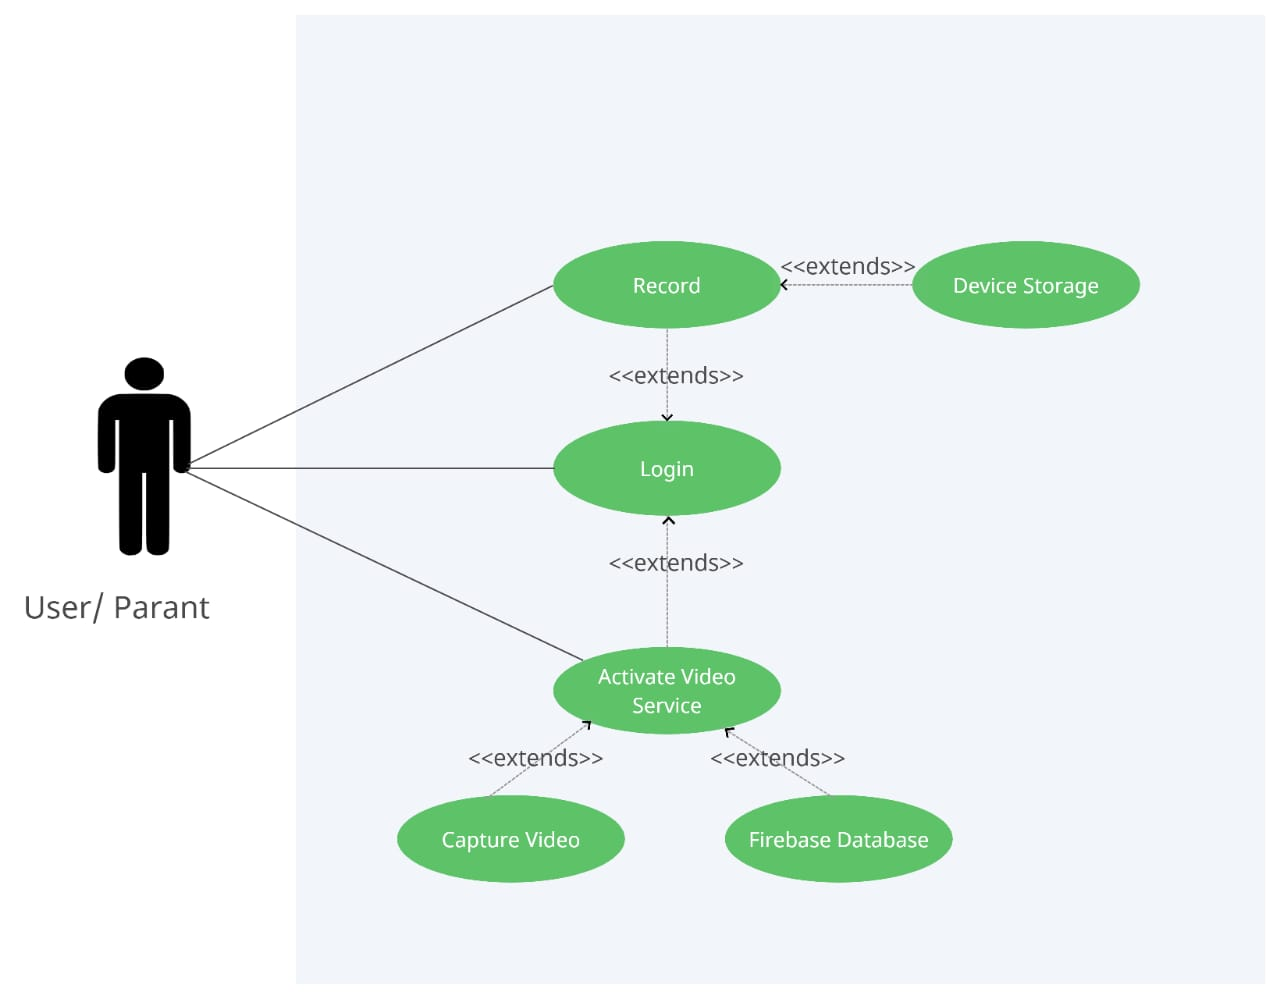
\includegraphics[width=1\textwidth]{b1.jpeg}
    \caption{Use case diagram}
    \label{Use case diagram}
\end{figure}

\subsection{Functional Requirements}
\par We need to add Functional requrements here.

\subsection{Non-Functional Requirements}
\par Non-functional requirements address aspects of the system other than the specific
functions it performs. These aspects include system performance, costs, and such
general system characteristics as reliability, security, and portability. The non-
functional requirements also address aspects of the system development process
and operational personnel. 
\par It includes the following:
\begin{itemize}
	\item The system was user friendly and consistent.
	\item The system provided attractive graphical interface for the user.
	\item The system allowed user access to installed environment.
	\item The system targeted customer base.
\end{itemize}

\subsection{System Requirements}
\par To be used efficiently, the RFID Based Surveillance System will need certain hard-
ware components and software resources to be present on a computer.\\
These requirements are regarded as minimum for the sake of running the system:

\subsectionfont{\normalsize}
\subsection*{Hardware Requirements}
\begin{itemize}
	\item Raspberry Pi 3B - 1.2GHz, Memory - 1GB RAM, 40-pin extended GPIO.
	\item RFID MF RC522 - 13.56MHz, Data Transfer Rate: Maximum 10Mbit/s 
\end{itemize}
\subsection*{Software Requirements}
\begin{itemize}
	\item Server - Python Localhost Server, DBMS - Firebase Realtime Database.
	\item Client - Android OS (Minimum api 29)
\end{itemize}
\subsectionfont{\large}

\section{System Design}
\par The new RFID Based Surveillance System has been designed in line with the
user and system requirements that were identified during the data collection and
analysis stage. The system will be used by the Parents and th School authority.

\subsection{Network and System Architecture}


